\documentclass[tikz]{standalone}
\usepackage{tikz}
\usetikzlibrary{arrows.meta, positioning, backgrounds, calc}

\begin{document}
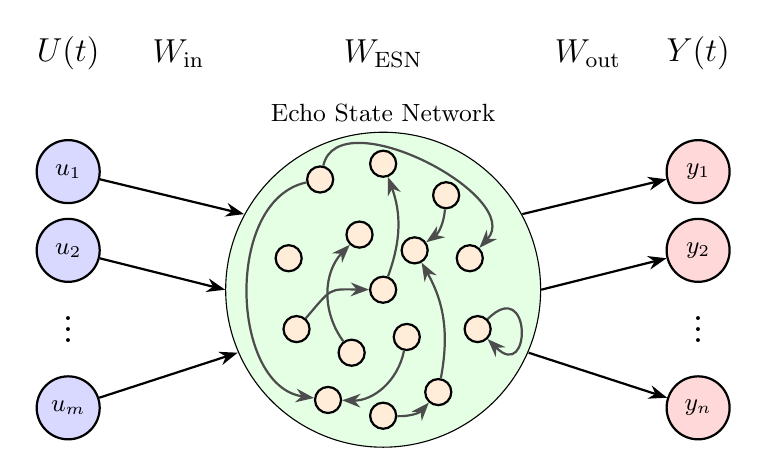
\begin{tikzpicture}[
    >=Stealth,
    thick,
    node distance=1.2cm,
    input node/.style={draw, circle, fill=blue!15, minimum size=0.8cm, font=\small},
    reservoir node/.style={
        draw, 
        circle, 
        fill=orange!15, 
        minimum size=0.3cm,  % Increased from inner sep=1pt
        font=\scriptsize
    },
    output node/.style={draw, circle, fill=red!15, minimum size=0.8cm, font=\small},
    connection/.style={->, black, thick},
    internal connection/.style={->, black!70}
]

% Title labels with more professional font sizes
\node at (0,3) {\large $U(t)$};
\node at (8,3) {\large $Y(t)$};

% Input nodes with consistent styling
\node[input node] (i1) at (0,1.5) {$u_1$};
\node[input node] (i2) at (0,0.5) {$u_2$};
\node at (0,-0.4) {$\LARGE \vdots$};  % Removed circle for vdots
\node[input node] (i4) at (0,-1.5) {$u_m$};

% Reservoir with subtle gradient effect
\begin{scope}[on background layer]
    \node[draw,circle,minimum size=4cm,fill=green!10,
          label={[font=\small]above:Echo State Network}] 
          (reservoir) at (4,0) {};
\end{scope}

% Internal reservoir nodes with better space utilization
\node[reservoir node] (r1) at (3.2, 1.4) {};  % Upper left
\node[reservoir node] (r2) at (4.0, 1.6) {};  % Upper middle
\node[reservoir node] (r3) at (4.8, 1.2) {};  % Upper right
\node[reservoir node] (r4) at (5.1, 0.4) {};  % Right upper
\node[reservoir node] (r5) at (5.2,-0.5) {};  % Right lower
\node[reservoir node] (r6) at (4.7,-1.3) {};  % Lower right
\node[reservoir node] (r7) at (4.0,-1.6) {};  % Lower middle
\node[reservoir node] (r8) at (3.3,-1.4) {};  % Lower left
\node[reservoir node] (r9) at (2.9,-0.5) {};  % Left lower
\node[reservoir node] (r10) at (2.8, 0.4) {}; % Left upper
\node[reservoir node] (r11) at (3.7, 0.7) {}; % Inner upper left
\node[reservoir node] (r12) at (4.4, 0.5) {}; % Inner upper right
\node[reservoir node] (r13) at (4.3,-0.6) {}; % Inner lower right
\node[reservoir node] (r14) at (3.6,-0.8) {}; % Inner lower left
\node[reservoir node] (r15) at (4.0, 0.0) {}; % Center

% Sparse random connections and self-connections
% Self connections (just one)
\draw[internal connection] (r5) to[out=45,in=-45,looseness=8] (r5);

% Sparse random connections across the network
\draw[internal connection] (r1) to[bend left=105] (r4);
\draw[internal connection] (r3) to[bend left=25] (r12);
\draw[internal connection] (r6) to[bend right=20] (r12);
\draw[internal connection] (r7) to[bend right=25] (r6);
\draw[internal connection] (r9) to[bend left=25, looseness=1.5] (r15);

% A few cross-connections for complexity
\draw[internal connection] (r15) to[bend right=20] (r2);
%\draw[internal connection] (r13) to[bend right=20] (r2);
\draw[internal connection] (r14) to[bend left=40] (r11);

% Just a couple long-range connections
\draw[internal connection] (r1) to[bend right=80] (r8);
\draw[internal connection] (r13) to[bend left=40] (r8);

% Output nodes with consistent styling
\node[output node] (o1) at (8,1.5) {$y_1$};
\node[output node] (o2) at (8,0.5) {$y_2$};
\node at (8,-0.4) {\LARGE $\vdots$};  % Removed circle for vdots
\node[output node] (o4) at (8,-1.5) {$y_n$};

% Input connections to reservoir edge
\draw[connection] (i1) -- ($(reservoir.west)+(0.12*2cm,0.8*1.2cm)$);
\draw[connection] (i2) -- ($(reservoir.west)+(0*2cm,0*2cm)$);
\draw[connection] (i4) -- ($(reservoir.west)+(0.08*2cm,-0.4*2cm)$);

% Output connections from reservoir edge
\draw[connection] ($(reservoir.east)+(-0.12*2cm,0.8*1.2cm)$) -- (o1);
\draw[connection] ($(reservoir.east)+(0*2cm,0*2cm)$) -- (o2);
\draw[connection] ($(reservoir.east)+(-0.08*2cm,-0.4*2cm)$) -- (o4);

% Weight labels with better positioning and font
\node[font=\large] at (1.4,3) {$W_{\mathrm{in}}$};
\node[font=\large] at (6.6,3) {$W_{\mathrm{out}}$};
\node[font=\large] at (4,3) {$W_{\mathrm{ESN}}$};

\end{tikzpicture}
\end{document}
